\let\negmedspace\undefined
\let\negthickspace\undefined
\documentclass[journal]{IEEEtran}
\usepackage[a5paper, margin=10mm, onecolumn]{geometry}
\usepackage{tfrupee} % Include tfrupee package

\setlength{\headheight}{1cm} % Set the height of the header box
\setlength{\headsep}{0mm}     % Set the distance between the header box and the top of the text

\usepackage{gvv-book}
\usepackage{gvv}
\usepackage{cite}
\usepackage{amsmath,amssymb,amsfonts,amsthm}
\usepackage{algorithmic}
\usepackage{graphicx}
\usepackage{textcomp}
\usepackage{xcolor}
\usepackage{txfonts}
\usepackage{listings}
\usepackage{enumitem}
\usepackage{mathtools}
\usepackage{gensymb}
\usepackage{comment}
\usepackage[breaklinks=true]{hyperref}
\usepackage{tkz-euclide} 
\usepackage{listings}
% \usepackage{gvv}                                        
\def\inputGnumericTable{}                                 
\usepackage[latin1]{inputenc}                                
\usepackage{color}                                            
\usepackage{array}                                            
\usepackage{longtable}                                       
\usepackage{calc}                                             
\usepackage{multirow}                                         
\usepackage{hhline}                                           
\usepackage{ifthen}                                           
\usepackage{lscape}
\begin{document}

\bibliographystyle{IEEEtran}
\vspace{3cm}

\title{8.3.4}
\author{EE24BTECH11013 - MANIKANTA D}
 \maketitle
% \newpage
% \bigskip
{\let\newpage\relax\maketitle}

\renewcommand{\thefigure}{\theenumi}
\renewcommand{\thetable}{\theenumi}
\setlength{\intextsep}{10pt} % Space between text and floats


\numberwithin{equation}{enumi}
\numberwithin{figure}{enumi}
\renewcommand{\thetable}{\theenumi}
\textbf{Question}:\\
Sketch the graph of $y = \abs{x + 3}$ and evaluate $\int_{-6}^{0} \abs{x + 3}dx$.
\\
\textbf{Solution: }\\
Integral to calculate, 
\begin{align}
    J = \int_{-6}^{0} \abs{x + 3}dx
\end{align}
Using the trapezoidal rule,
\begin{align}
    J = \int_a^b f(x)dx \approx h \left(\frac{1}{2}f(x_0) + f(x_1) + f(x_2) + \cdots + f(x_{n-1}) + \frac{1}{2}f(x_n)\right)
\end{align}
Recursive formula for the numerical solution:
\begin{align}
    J = j_n, \text{ where } j_{i+1} = j_i + h \frac{f(x_{i+1}) + f(x_i)}{2}, \\
    x_{i+1} = x_i + h.
\end{align}
\begin{align}
    j_{i+1} = j_i + h \frac{\abs{x_{i+1} + 3} + \abs{x_i + 3}}{2}, \\
    x_{i+1} = x_i + h.
\end{align}
where $h = \frac{b-a}{n}$, and $x_i = a + ih$.\\
Let $a = -6$, $b = 0$, and $f(x) = \abs{x + 3}$. Choose $n = 8$, so:
\begin{align}
    h = \frac{0 - (-6)}{8} = \frac{6}{8} = 0.75.
\end{align}
The points are:
\begin{align}
    x_0 = -6, \, x_1 = -5.25, \, x_2 = -4.5, \, x_3 = -3.75, \, x_4 = -3, \, \\
    x_5 = -2.25, \, x_6 = -1.5, \, x_7 = -0.75, \, x_8 = 0.
\end{align}
The corresponding function values are:
\begin{align}
    f(x_0) = \abs{-6 + 3} = 3, \, f(x_1) = \abs{-5.25 + 3} = 2.25, \, f(x_2) = \abs{-4.5 + 3} = 1.5, \\
    f(x_3) = \abs{-3.75 + 3} = 0.75, \, f(x_4) = \abs{-3 + 3} = 0, \, \\
    f(x_5) = \abs{-2.25 + 3} = 0.75, \, f(x_6) = \abs{-1.5 + 3} = 1.5, \, \\
    f(x_7) = \abs{-0.75 + 3} = 2.25, \, f(x_8) = \abs{0 + 3} = 3.
\end{align}
Substitute into the trapezoidal rule formula:
\begin{align}
    J \approx 0.75 \left(\frac{1}{2}f(x_0) + f(x_1) + f(x_2) + f(x_3) + f(x_4) + f(x_5) + f(x_6) + f(x_7) + \frac{1}{2}f(x_8)\right) \\
    J \approx 0.75 \left(\frac{1}{2}(3) + 2.25 + 1.5 + 0.75 + 0 + 0.75 + 1.5 + 2.25 + \frac{1}{2}(3)\right) \\
    J \approx 0.75 \left(1.5 + 2.25 + 1.5 + 0.75 + 0 + 0.75 + 1.5 + 2.25 + 1.5\right) \\
    J \approx 0.75 \times 12 \times 2 = 18.
\end{align}
The approximate value of the integral using the trapezoidal rule with $n = 8$ is $J \approx 18$.

\textbf{Theoretical Solution:}\\
Using the properties of the absolute value function, split the integral at $x = -3$:
\begin{align}
    J = \int_{-6}^{-3} -(x + 3) dx + \int_{-3}^{0} (x + 3) dx.
\end{align}
Evaluate each part:
\begin{align}
    \int_{-6}^{-3} -(x + 3) dx &= \int_{-6}^{-3} (-x - 3) dx = \left[-\frac{x^2}{2} - 3x\right]_{-6}^{-3} = \frac{27}{2}, \\
    \int_{-3}^{0} (x + 3) dx &= \left[\frac{x^2}{2} + 3x\right]_{-3}^{0} = \frac{9}{2}.
\end{align}
Combine results:
\begin{align}
    J = \frac{27}{2} + \frac{9}{2} = \frac{36}{2} = 18.
\end{align}
The exact value of the integral is $J = 18$.

\begin{figure}[h]
    \centering
    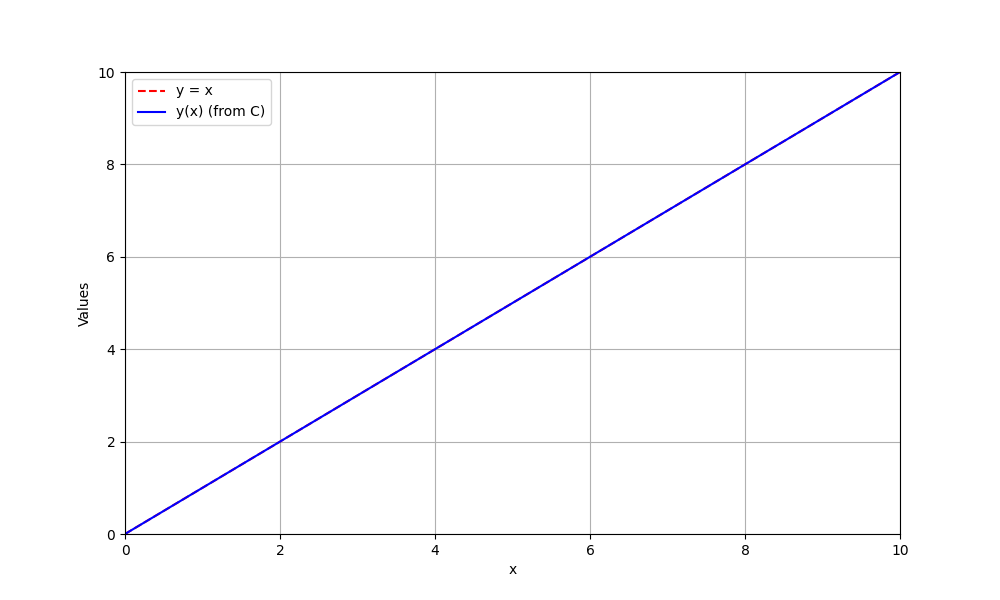
\includegraphics[width=\columnwidth]{fig.png}
    \caption{Plot of the differential equation}
    \label{fig:Plot}
    \end{figure}
    \end{document}
